% Lecture Template for ME3050-001-Tristan Hill - Spring 2020
% 
% Dynamics Modeling and Controls
% Dyanmics Review


% Document settings
\documentclass[11pt]{article}
\usepackage[margin=1in]{geometry}
\usepackage[pdftex]{graphicx}
\usepackage{multirow}
\usepackage{setspace}
\usepackage{hyperref}
\usepackage{color,soul}
\usepackage{fancyvrb}
\usepackage{framed}
\usepackage{wasysym}
\usepackage{multicol}

\pagestyle{plain}
\setlength\parindent{0pt}
\hypersetup{
    bookmarks=true,         % show bookmarks bar?
    unicode=false,          % non-Latin characters in Acrobat’s bookmarks
    pdftoolbar=true,        % show Acrobat’s toolbar?
    pdfmenubar=true,        % show Acrobat’s menu?
    pdffitwindow=false,     % window fit to page when opened
    pdfstartview={FitH},    % fits the width of the page to the window
    pdftitle={My title},    % title
    pdfauthor={Author},     % author
    pdfsubject={Subject},   % subject of the document
    pdfcreator={Creator},   % creator of the document
    pdfproducer={Producer}, % producer of the document
    pdfkeywords={keyword1} {key2} {key3}, % list of keywords
    pdfnewwindow=true,      % links in new window
    colorlinks=true,       % false: boxed links; true: colored links
    linkcolor=red,          % color of internal links (change box color with linkbordercolor)
    citecolor=green,        % color of links to bibliography
    filecolor=magenta,      % color of file links
    urlcolor=blue           % color of external links
}

% assignment number 
\newcommand{\NUM}{1 } 
\newcommand{\VSpaceSize}{2mm} 
\newcommand{\HSpaceSize}{2mm} 

\newcommand{\B}{\color{blue}} 
\newcommand{\K}{\color{black}}
%\newcommand{\B}{\color{blue}} 

\definecolor{mygray}{rgb}{.6, .6, .6}

\setulcolor{red} 
\setstcolor{green} 
\sethlcolor{mygray} 

\begin{document}

\textbf{ \LARGE ME 3050 Lecture - Dynamics Review - Lecture \NUM  } \\

\begin{itemize}



	\item \textbf{ \Large The \B dynamics \K are represented as ordinary \vspace{3mm}\\
differential equations called the \\\\ \underline{\hspace{60mm}} of \underline{\hspace{60mm}}.} \vspace{2mm}\\

	\item \textbf{ \Large Deriving the 	\underline{\hspace{60mm}} of \underline{\hspace{60mm}} \vspace{1mm}\\is typically done in one of two ways.} \\
\Large
	\begin{enumerate}
		\item Newtonian Approach - Vector Based Method \vspace{3mm}\\
		\begin{itemize}
\item Translational\\
\item Rotational  \vspace{10mm}\\
\end{itemize} 
\item Conservation of Energy Approach - Energy Based Method \vspace{3mm}\\
		\begin{itemize}
\item Kinetic Energy\\
\item Potential Energy\\  
\end{itemize} 
	\end{enumerate}

\newpage

\item \textbf{ \Large  Example:} DJI Phantom with 3-axis Camera Gimbal - Whoa!!!\\

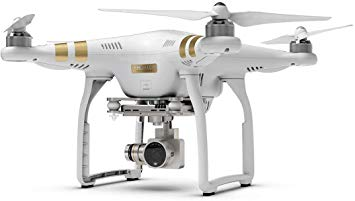
\includegraphics[scale=1]{dji_phantom.jpg}


\newpage

\item \textbf{ \Large  Simpler Example:} Quarter Car Suspension Model\\

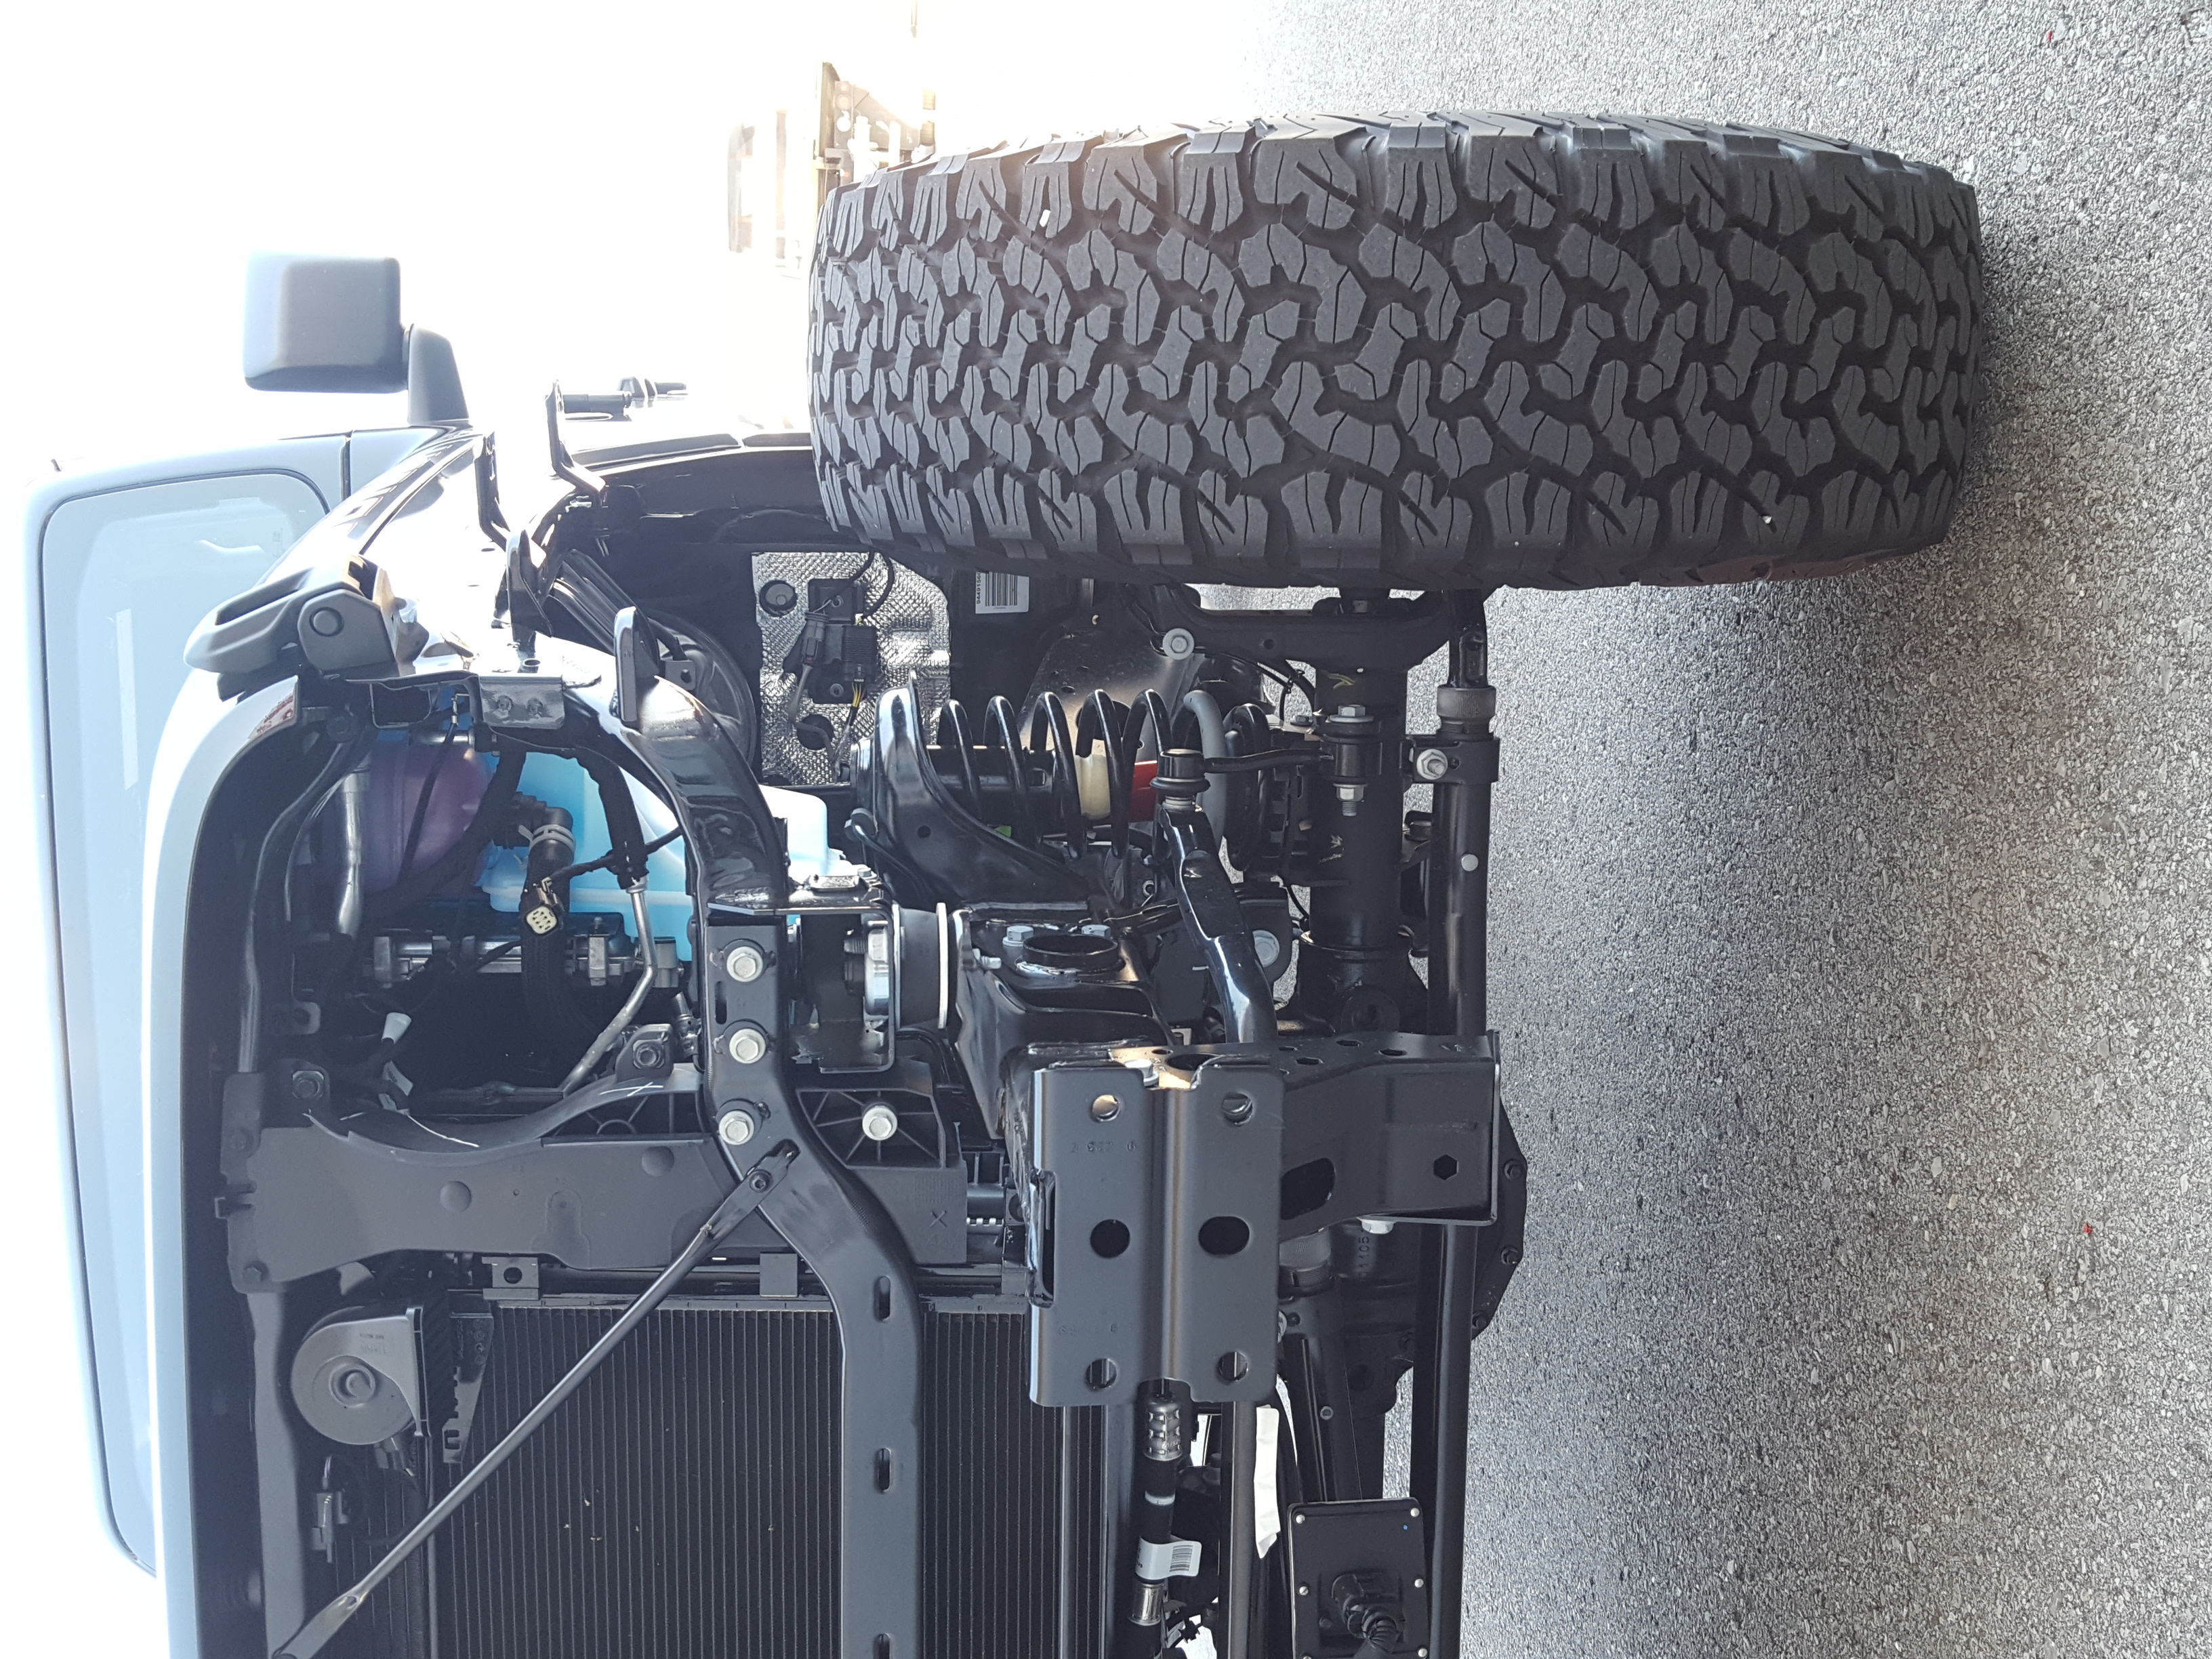
\includegraphics[scale=.1,angle=-90,origin=c]{jeep_01.jpg} 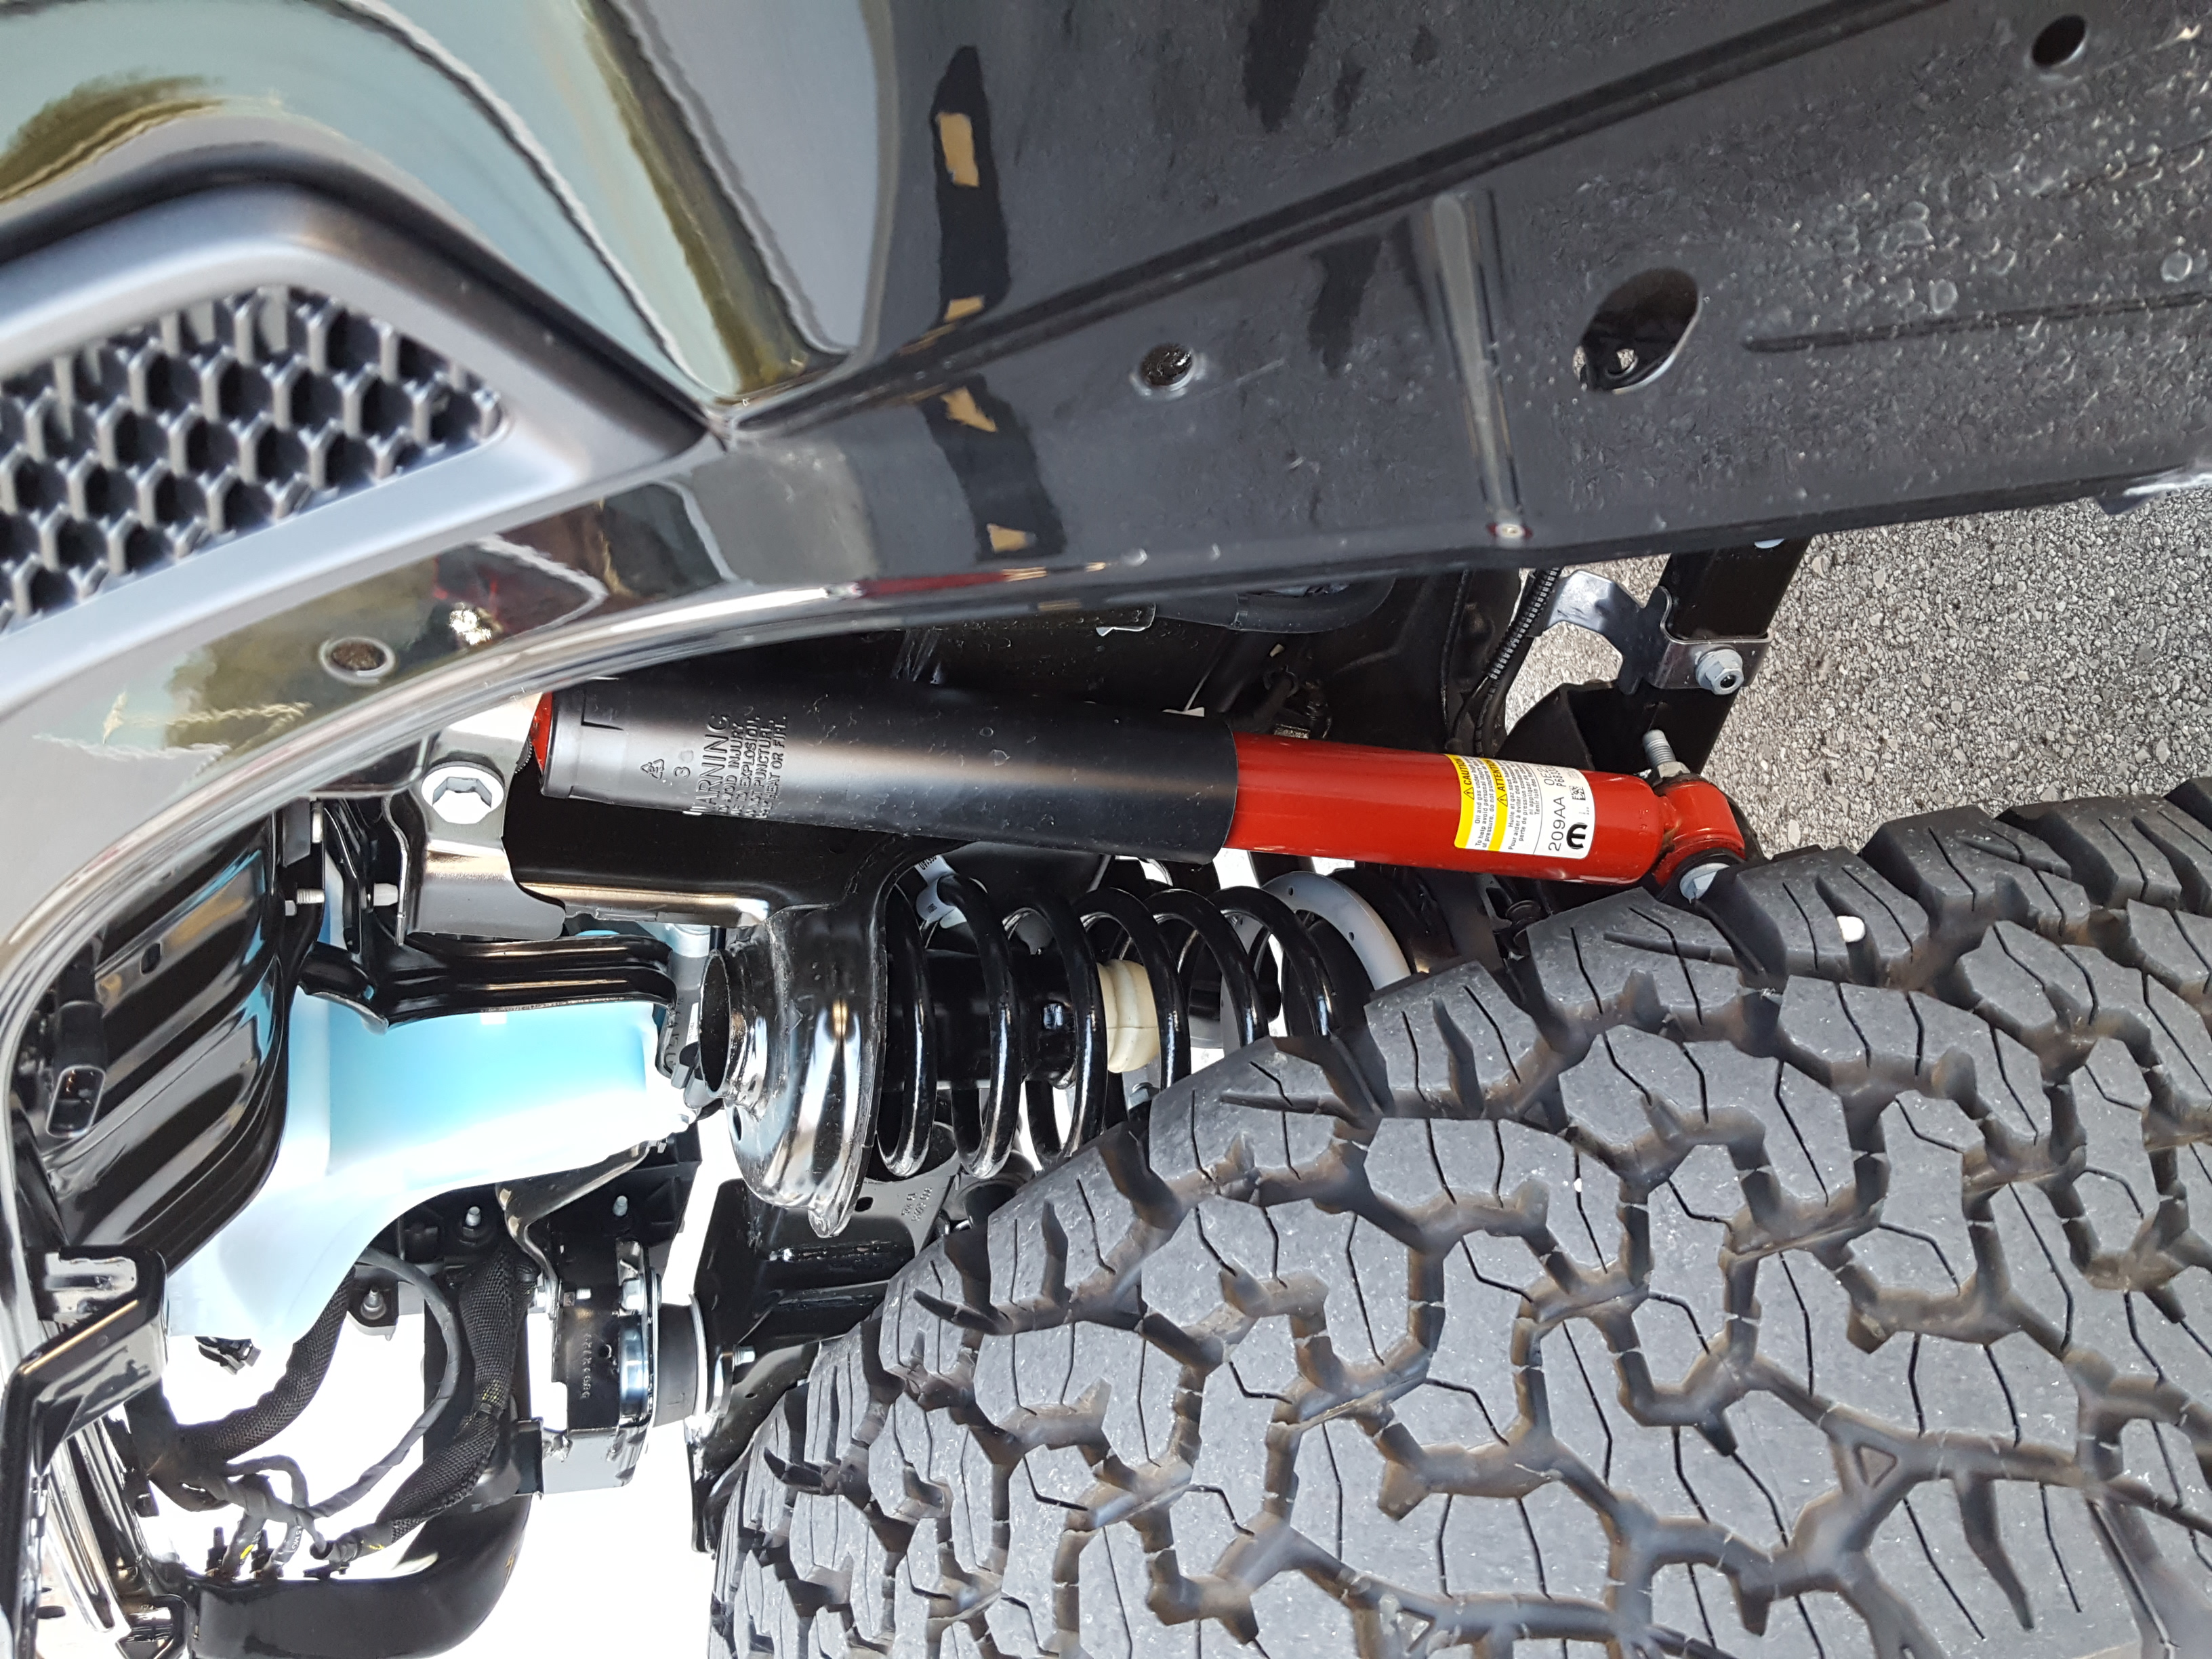
\includegraphics[scale=.1,angle=-90,origin=c]{jeep_02.jpg} \\
\begin{itemize}
\item \textbf{ \Large \underline{Problem Statement} -  Derive the \B equations of motion \K using (1) Newton's approach and validate using the (2) Conservation of Energy.}\\

\item \textbf{ \Large \underline{Assumptions} - List the assumptions used in the modeling process.  } 


\newpage

\item \textbf{ \Large \underline{Figure(s)} - Draw a \B free body diagram (FBD) \K and/or a sketch of the system. Some problems will require more than one. You need at least one per \B degree of freedom \K.} 

\newpage

\item \textbf{ \Large \underline{Newton's Approach} }\\
\begin{enumerate}
\item Draw a Free Body Diagram \vspace{20mm}\\
\item Determine all \B forces \K acting on the system and their \B directions\K. \vspace{20mm}\\
\item Write \B Newton's second law \K for the appropriate DOF. \vspace{70mm}\\
\item Re-write the ODE in the \B standard form \K of a system equation.
\end{enumerate}

\newpage
\item \textbf{ \Large \underline{Conservation of Energy Approach} }\\
\begin{enumerate}
\item Draw a Free Body Diagram \vspace{20mm}\\
\item Determine all \B energies \K present in the system and their \B type\K. \vspace{20mm}\\
\newpage
\item Write \B Conservation of Energy \K for system. Call this {\it equation 1}.\vspace{70mm}\\
\item Take the derivative of {\it equation 1} with respect to time. Set this equal to zero and call this {\it equation 2}. \vspace{70mm}\\
\item Re-write the ODE in the \B standard form \K of a system equation.
\end{enumerate}


\end{itemize}


\end{itemize}


	

\end{document}



